\documentclass[tikz,border=12pt]{standalone}
\usepackage[T1]{fontenc}
\usepackage[scaled]{helvet}
\renewcommand{\familydefault}{\sfdefault}
\usetikzlibrary{positioning,arrows.meta,shapes.geometric,calc}

% ---------- Colors ----------
\definecolor{pretrainC}{RGB}{52,101,164}   % pretraining stage
\definecolor{finetuneC}{RGB}{206,92,0}     % finetuning stage
\definecolor{capC}{RGB}{78,154,6}          % emergent capabilities
\definecolor{noteC}{RGB}{60,60,60}

\tikzset{
	box/.style={draw, rounded corners=8pt, line width=1pt, align=left,
		inner sep=8pt, font=\small},
	flow/.style={-{Latex[length=3.5mm,width=3mm]}, line width=1.8pt},
	steplabel/.style={font=\small\bfseries, above=2pt},
	caption/.style={align=center, font=\small},
	note/.style={align=center, font=\footnotesize\bfseries, text=noteC},
	pointer/.style={-{Latex[length=2mm]}, thin, noteC},
	% ----- Icons -----
	pics/document/.style={code={
			\foreach \d in {0.16,0.08,0}{
				\filldraw[fill=white, draw=black, line width=0.7pt]
				($(-0.4,-0.5)+(-\d,\d)$) -- ++(0,1) -- ++(0.55,0) -- ++(0.25,-0.25)
				-- ++(0,-0.75) -- cycle;
			}
			\draw[line width=0.7pt] (0.15,0.5) -- (0.15,0.25) -- (0.4,0.25);
			\foreach \y in {0.15,0,-0.15,-0.3}
			\draw[line width=0.6pt] (-0.28,\y) -- (0.28,\y);
	}},
	pics/house/.style={code={
			\draw[line width=1.3pt, line join=round]
			(-0.55,-0.6) -- (-0.55,0.15) -- (-0.75,0.15) -- (0,0.75)
			-- (0.75,0.15) -- (0.55,0.15) -- (0.55,-0.6) -- cycle;
			\draw[line width=1.3pt] (-0.18,-0.6) -- (-0.18,-0.15)
			arc[start angle=180, end angle=0, radius=0.18] -- (0.18,-0.6);
	}},
	pics/bulb/.style={code={
			\draw[line width=1pt, fill=yellow!25] (0,0.1) circle[radius=0.35];
			\draw[line width=1pt, fill=white] (-0.15,-0.25) rectangle (0.15,-0.5);
			\draw[line width=0.8pt] (-0.15,-0.33) -- (0.15,-0.33)
			(-0.15,-0.42) -- (0.15,-0.42);
			\foreach \a in {90,135,45,180,0}
			\draw[line width=1pt] ($(0,0.1)+(\a:0.5)$) -- ($(0,0.1)+(\a:0.7)$);
	}},
}

\begin{document}
	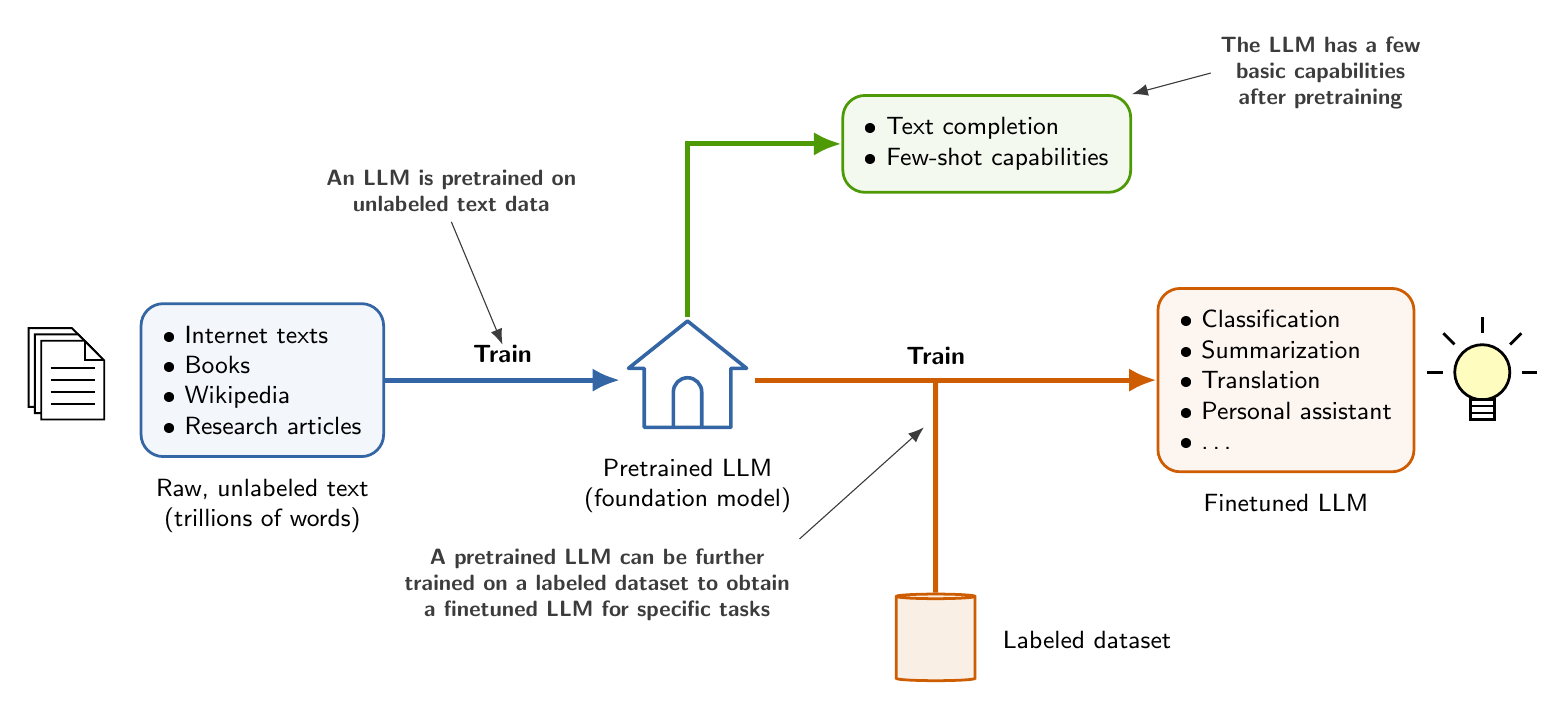
\begin{tikzpicture}
		
		% ================= Stage 1: raw data =================
		\node[box, draw=pretrainC, fill=pretrainC!6] (raw) at (0,0)
		{\textbullet~Internet texts\\
			\textbullet~Books\\
			\textbullet~Wikipedia\\
			\textbullet~Research articles};
		\pic at ($(raw.west)+(-0.85,0)$) {document};
		\node[caption, below=4pt of raw] {Raw, unlabeled text\\(trillions of words)};
		
		% ================= Stage 2: pretrained LLM =================
		\node[minimum width=1.7cm, minimum height=1.6cm] (pre) at (5.4,0) {};
		\pic[pretrainC] at (pre.center) {house};
		\node[caption, below=2pt of pre] {Pretrained LLM\\(foundation model)};
		
		% Pretraining arrow
		\draw[flow, pretrainC] (raw.east) -- node[steplabel, text=black] {Train}
		coordinate[pos=0.5] (trainA) (pre.west);
		
		% ================= Basic capabilities after pretraining =================
		\node[box, draw=capC, fill=capC!6] (cap) at (9.2,3.0)
		{\textbullet~Text completion\\
			\textbullet~Few-shot capabilities};
		\draw[flow, capC] (pre.north) |- (cap.west);
		
		% ================= Stage 3: finetuned LLM =================
		\node[box, draw=finetuneC, fill=finetuneC!6] (fine) at (13.0,0)
		{\textbullet~Classification\\
			\textbullet~Summarization\\
			\textbullet~Translation\\
			\textbullet~Personal assistant\\
			\textbullet~\dots};
		\pic at ($(fine.east)+(0.85,0)$) {bulb};
		\node[caption, below=4pt of fine] {Finetuned LLM};
		
		% Finetuning arrow with labeled dataset merging in
		\coordinate (join) at ($(pre.east)!0.45!(fine.west)$);
		\draw[flow, finetuneC] (pre.east) -- (fine.west);
		\node[steplabel] at (join) {Train};
		
		\node[cylinder, shape border rotate=90, aspect=0.25, draw=finetuneC,
		fill=finetuneC!10, line width=1pt, minimum width=1cm,
		minimum height=1.1cm] (db) at ($(join)+(0,-3.3)$) {};
		\node[caption, right=6pt of db] {Labeled dataset};
		\draw[line width=1.8pt, finetuneC] (db.north) -- (join);
		
		% ================= Annotations =================
		\node[note] (n1) at (2.4,2.4)
		{An LLM is pretrained on\\unlabeled text data};
		\draw[pointer] (n1.south) -- ($(trainA)+(0,0.45)$);
		
		\node[note, anchor=west] (n2) at ($(cap.east)+(1.0,0.9)$)
		{The LLM has a few\\basic capabilities\\after pretraining};
		\draw[pointer] (n2.west) -- (cap.north east);
		
		\node[note] (n3) at ($(join)+(-4.3,-2.6)$)
		{A pretrained LLM can be further\\trained on a labeled dataset to obtain\\a finetuned LLM for specific tasks};
		\draw[pointer] (n3.north east) -- ($(join)+(-0.15,-0.6)$);
		
	\end{tikzpicture}
\end{document}